\begin{example}
Να διπλασιαστεί το μήκος των πλευρών του τριγώνου με κορυφές $A(0,0)$, $B(1,1)$ και $C(5,2)$ διατηρώντας την κορυφή $C(5,2)$ σταθερή.
\end{example}
\begin{solution}
	

\begin{figure}[h!]
	\begin{center}
		\begin{minipage}[b]{0.45\textwidth} % Top-left image
		    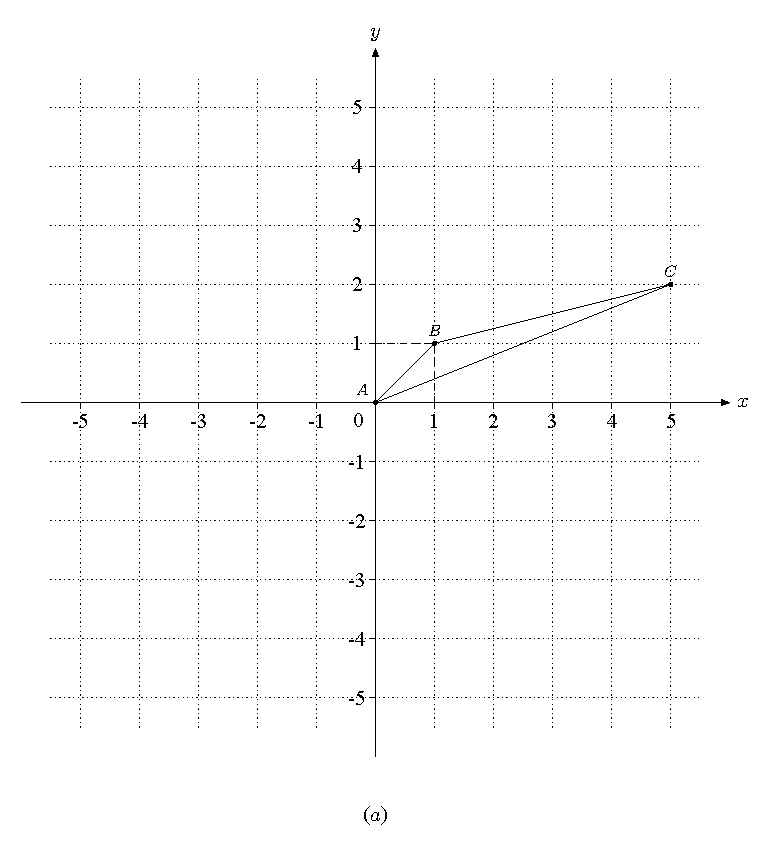
\includegraphics[width=\textwidth]{Chapter2/figure15a.pdf}
		\end{minipage}%
	\hfill
		\begin{minipage}[b]{0.4\textwidth} % Top-right image
		    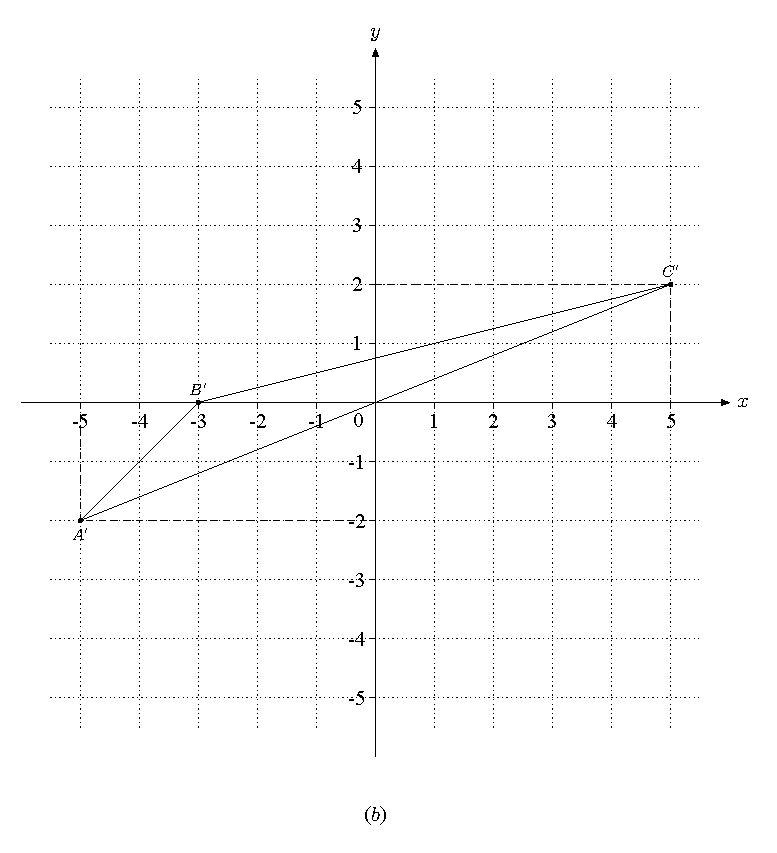
\includegraphics[width=\textwidth]{Chapter2/figure15b.pdf}
		\end{minipage}
	\end{center}
%\caption{Στρέβλωση ενός τετραγώνου για $a=2$ και $b=2$}
\end{figure}


\begin{tabular}{m{0.6\textwidth}m{0.5\textwidth}}
	Αρχικό μήκος πλευράς $BC$: & $\sqrt{(5-1)^2 + (2-1)^2} = \sqrt{17}$ \\
	Μεγεθυνόμενο το τρίγωνο του (σχήματος) γίνεται: & \\
	Τελικό μήκος πλευράς $BC'$: & $\sqrt{(5-(-3))^2 + (2-0)^2} = 2 \sqrt{17}$
\end{tabular}


Από το παράδειγμα 3 χρησιμοποιούμε τον πίνακα $S_{a,b,p}$ όπου $a=b=2$ και $P=C(5,2)$. Στην προκείμενη περίπτωση το διάνυσμα μεταφοράς είναι $v=5\hat{i}+2\hat{j}$ (σχήμα 3.15 (a)). Ο πίνακας $S_{2,2,C}$ παίρνει την ακόλουθη τιμή:

\[
S_{2,2,C} = \begin{bmatrix}
2 & 0 & -5 \\
0 & 2 & -2 \\
0 & 0 & 1
\end{bmatrix}
\]

Επιδρούμε με τον πίνακα $S_{2,2,C}$ πάνω στο τρίγωνο $ABC$ και προκύπτει:

\[
A'B'C' = S_{2,2,C} \cdot ABC = \begin{bmatrix}
2 & 0 & -5 \\
0 & 2 & -2 \\
0 & 0 & 1
\end{bmatrix} \cdot \begin{bmatrix}
0 & 1 & 5 \\
0 & 1 & 2 \\
1 & 1 & 1
\end{bmatrix} = \begin{bmatrix}
-5 & -2 & 5 \\
-2 & 0 & 2 \\
1 & 1 & 1
\end{bmatrix}
\]

Τελικά οι συντεταγμένες του καινούργιου τριγώνου δίνονται από τις σχέσεις:
\[
A' = (-5, -2), \quad B' = (-3, 0), \quad C' = (5, 2)
\]

\end{solution}